\chapter{Electrical Power}
\label{chapter:electrical-power}

This chapter describes the electrical power system in the {\projectname} installation. The electrical grounding system is described in Chapter~\ref{chapter:electrical-grounding}.

Figure~\ref{figure:schematic-electrical-power}
shows a schematic of the electrical power system. The sections below describe each part in detail.

TODO: Don’t know which DDOTI circuits are L1-N, L2-N, or L3-N.

\begin{figure*}[p]
\begin{center} 
\resizebox{\columnwidth}{!}{
\begin{tikzpicture}
[
 thick,
 >={latex},
 box/.style={
  inner sep=1mm,
  draw=black,
  rectangle,
  minimum width=2cm,
  minimum height=0.6cm,
  align=center
 },
 circuit/.style={
  draw=black,
  rectangle,
  fill=white
 }
]

\ifcoatli
\node at (-6,-3) [box,minimum width=12cm,right] (oan) {OAN Grid};
\node at (-6,-1) [box,minimum width=12cm,right] (transformer) {Isolation Transformer};
\node at (-6,0) [box,minimum width=12cm,right] (main-breaker-box) {Main Breaker Box};
\fi
\ifddoti
\node at (-6,-2) [box,minimum width=12cm,right] (oan) {OAN Grid};
\node at (-6,-1) [box,minimum width=12cm,right] (transformer) {Isolation Transformer};
\node at (-6,1) [box,minimum width=12cm,right] (main-breaker-box) {Main Breaker Box};
\fi
\node at (-6,2) [box,minimum width=12cm,right] (circuit-box) {Circuit Box};
\draw[->] (oan) -- (transformer);
\draw[->] (transformer) -- (main-breaker-box);
\draw[->] (main-breaker-box) -- (circuit-box);

\node at (-5,+4) [box] (socket-a) {Socket A};
\node at (+3.5,+5) [box] (lights) {Lights};
\node at (+1,+9) [box] (mount) {Mount};
\node at (-0.75,+4) [box] (socket-b) {Socket B};
\node at (+2,+4) [box] (sockets-d) {Sockets D};
\node at (+5,+4) [box] (socket-f) {Socket F};
\node at (-0.75,+5) [box] (ups-127) {127 V UPS};
\node at (-2,+6) [box] (ibb-127) {127 V iBB};
\node at (-5,+5) [box] (ups-220) {220 V UPS};
\node at (-5,+6) [box] (ibb-220) {220 V iBB};
\node at (-6,+7.5) [box,left] (enclosure) {Enclosure};
\ifcoatli
\node at (-6,+8.5) [box,left] (secondary) {Secondary};
\fi
\node at (+0,+7) [box,right] (rack-power-strip) {Rack Power Strip};
\node at (+0,+8) [box,right] (other-shed-electronics) {Other Shed Electronics};
\node at (+2,+6) [box] (fans-and-heater) {Fans and Heater};
\node at (+1,+11) [box,right] (platform-box) {Platform Box};
\ifcoatli
\node at (+1,+13) [box,right] (instrument-box) {Instrument Box};
\fi
\ifddoti
\node at (-1,+13) [box,right] (instrument0-box) {Instrument0 Box};
\node at (+3,+13) [box,right] (instrument1-box) {Instrument1 Box};
\fi
\node at (-3.0,+11) [box] (power-box) {Power Box};

\draw[->] 
 ($(circuit-box.north) + (-5.0,0)$) 
 -- node [circuit] {\scriptsize A} +(0,1)
 -- (socket-a);
\draw[->] 
 ($(circuit-box.north) + (-3.5,0)$) 
 -- node [circuit] {\scriptsize C} +(0,1)
 -- ($(power-box.south) + (-0.5,0)$);
\draw[->] 
 ($(circuit-box.north) + (-0.75,0)$) 
 -- node [circuit] {\scriptsize B} +(0,1)
 -- (socket-b.south);
\draw[->]
 ($(circuit-box.north) + (2,0)$) 
 -- node [circuit] {\scriptsize D} +(0,1)
 -- (sockets-d.south);
\draw[->] 
 ($(circuit-box.north) + (3.5,0)$) 
 -- node [circuit] {\scriptsize E} +(0,1)
 -- (lights.south);
\draw[->] 
 ($(circuit-box.north) + (5.0,0)$) 
 -- node [circuit] {\scriptsize F} +(0,1)
 -- (socket-f.south);

\draw[->] (socket-a) -- (ups-220);
\draw[->] (ups-220) -- (ibb-220);
\draw[->] 
 ($(ibb-220.north) + (-0.3,0)$)
 -- node [circuit] {\scriptsize A} +(0,1) 
 |- (enclosure.east);
\ifcoatli
\draw[->] 
 ($(ibb-220.north) + (+0.3,0)$)
 -- node [circuit] {\scriptsize A} +(0,1) 
 |- (secondary.east);
\fi

\draw[->] (socket-b) -- (ups-127);
\draw[->] ($(ups-127.north) + (-0.75,0)$) -- ($(ibb-127.south) + (+0.50,0)$);
\draw[->] ($(ups-127.north) + (-0.50,0)$) -- ($(ibb-127.south) + (+0.75,0)$);
\draw[->] ($(ups-127.north) + (+0.50,0)$) -- node [circuit] {\scriptsize B} +(0,1) |- (rack-power-strip.west);

\draw[->] 
 ($(ibb-127.north) + (-0.75,0)$)
 -- node [circuit] {\scriptsize B1} +(0,1)
 -- +(0,2)
 -| ($(power-box.south) + (+0.0,0)$);
\draw[->] 
 ($(ibb-127.north) + (-0.25,0)$)
 -- node [circuit] {\scriptsize B2} +(0,2)
 -- +(0,2.5)
 -| ($(power-box.south) + (+0.5,0)$);
\draw[->] 
 ($(ibb-127.north) + (+0.25,0)$) 
 -- node [circuit] {\scriptsize B} +(0,1)
 |- (mount.west);
\draw[->] 
 ($(ibb-127.north) + (+0.75,0)$) 
 -- node [circuit] {\scriptsize B} +(0,1)
 |- (other-shed-electronics.west);

\draw[->] 
 ($(power-box.east) + (0,-0.15)$)
 -- node [circuit] {\scriptsize B1} +(1,0)
 -- ($(platform-box.west) + (0,-0.15)$);
\draw[->] 
 ($(power-box.east) + (0,+0.15)$)
 -- node [circuit] {\scriptsize C} +(2.5,0)
 -- ($(platform-box.west) + (0,+0.15)$);

\ifcoatli
\draw[->] 
  (power-box.north) 
  -- node [circuit] {\scriptsize B2} +(0,0.7) 
  |- (instrument-box);
\fi
\ifddoti
\draw[->] 
  (power-box.north) 
  -- node [circuit] {\scriptsize B2} +(0,0.7) 
  |- (instrument0-box);
\draw[->] 
  (instrument0-box.east) 
  -- node [circuit] {\scriptsize B2} +(0.7,0) 
  |- (instrument1-box);
\fi

\draw[->] 
 (sockets-d.north) 
 -- node [circuit] {\scriptsize D} +(0,1)
 -- (fans-and-heater.south);

\draw[dashed] (-8,+10) -- (6.5,+10);
\draw[dashed] (-8,+12) -- (6.5,+12);
\draw[dashed] (-8,+14) -- (6.5,+14);
\node at (-8,+11) [right] {\normalsize Platform};
\node at (-8,+13) [right] {\normalsize Telescope};
\node at (-8,+6) [right] {\normalsize Shed};
\ifcoatli
\draw[dashed] (-8,-2) -- (6.5,-2);
\draw[dashed] (-8,+1) -- (6.5,+1);
\node at (-8,-0.5) [right] {\normalsize 84-cm};
\fi
\ifddoti
\draw[dashed] (-8,0) -- (6.5,0);
\fi

\end{tikzpicture}
}
\end{center}
\caption{Schematic of the Distribution of Electrical Power. The letters A to F refer to circuits.}
\label{figure:schematic-electrical-power}
\end{figure*}

\section{External Mains Supply}

The OAN electricity supply is 220~V 60~Hz three-phase.

\ifcoatli
The {\projectname} installation is connected to the OAN electricity supply via a spur to the circuit box in the 84-cm telescope building. This spur carries two phases (L1 and L2) and neutral (N). The phases are protected by an 80 A breaker. The circuit box and the breaker are shown in Figure~\ref{figure:main-breaker-box}.

\begin{figure}[t]
\begin{center}
\begin{labeled}{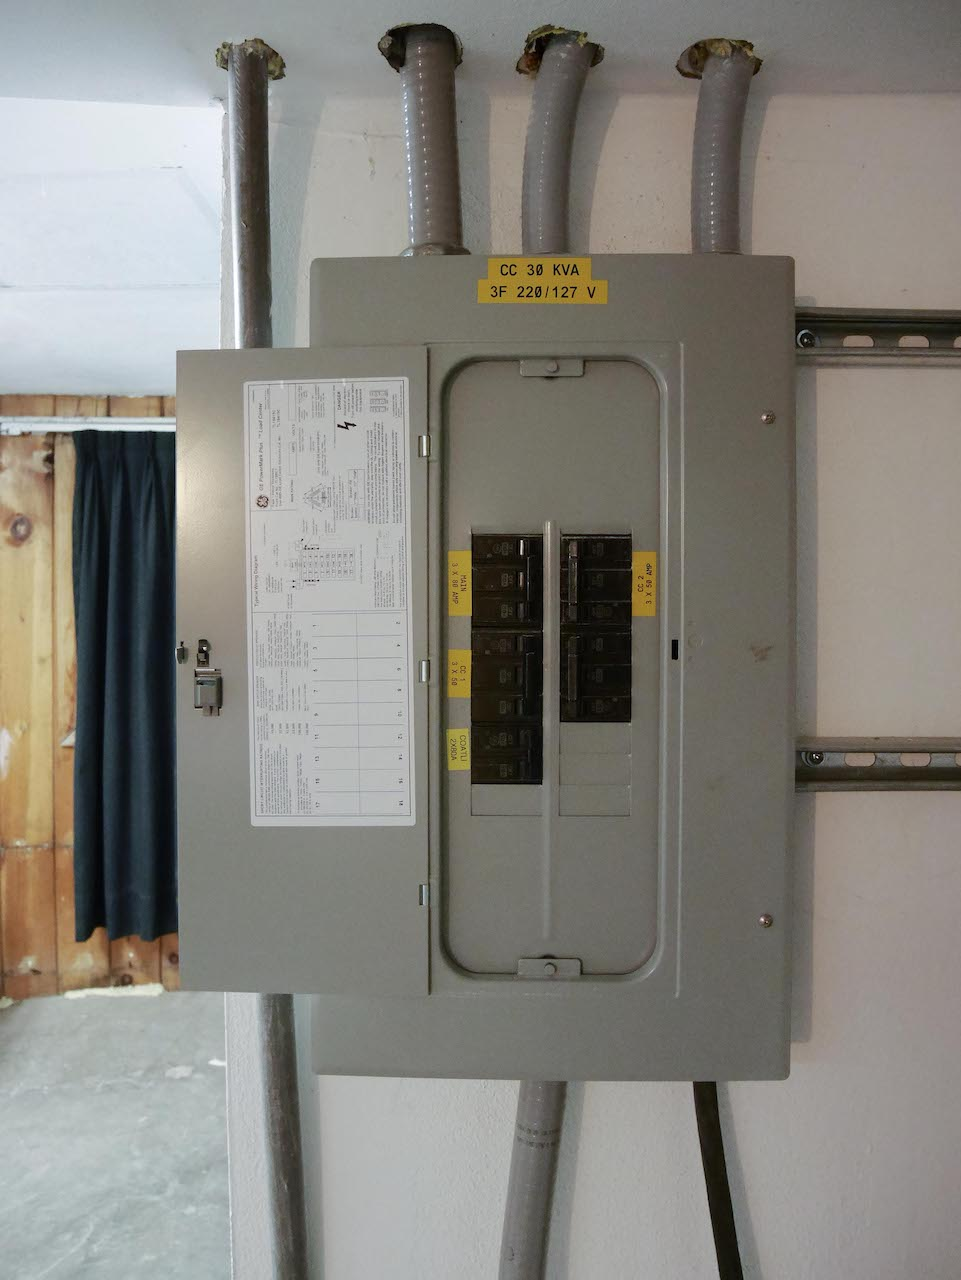
\includegraphics[height=0.7\linewidth]{figures/electrical-power-coatli-main-breaker-box.jpg}}
\arrowandlabel{(0.2,-1.0)}{(0,-5)}{north}{{\projectname} Main breaker}
\end{labeled}
\end{center}
\caption{The main breaker box in the 84-cm telescope building. The main breaker for the {\projectname} spur are at the lower left.}
\label{figure:main-breaker-box}
\end{figure}
\fi

\ifddoti
The {\projectname} installation is connected to the OAN electricity supply via an isolation transformer (on the north wall of the shed). This spur carries three phases (L1, L2, and L3) and neutral (N). The phases are protected by a 70~A breaker on a 30 kVA main breaker box inside the shed. The main breaker box is shown in Figure~\ref{figure:main-breaker-box}.

\begin{figure}[t]
\begin{center}
\begin{labeled}{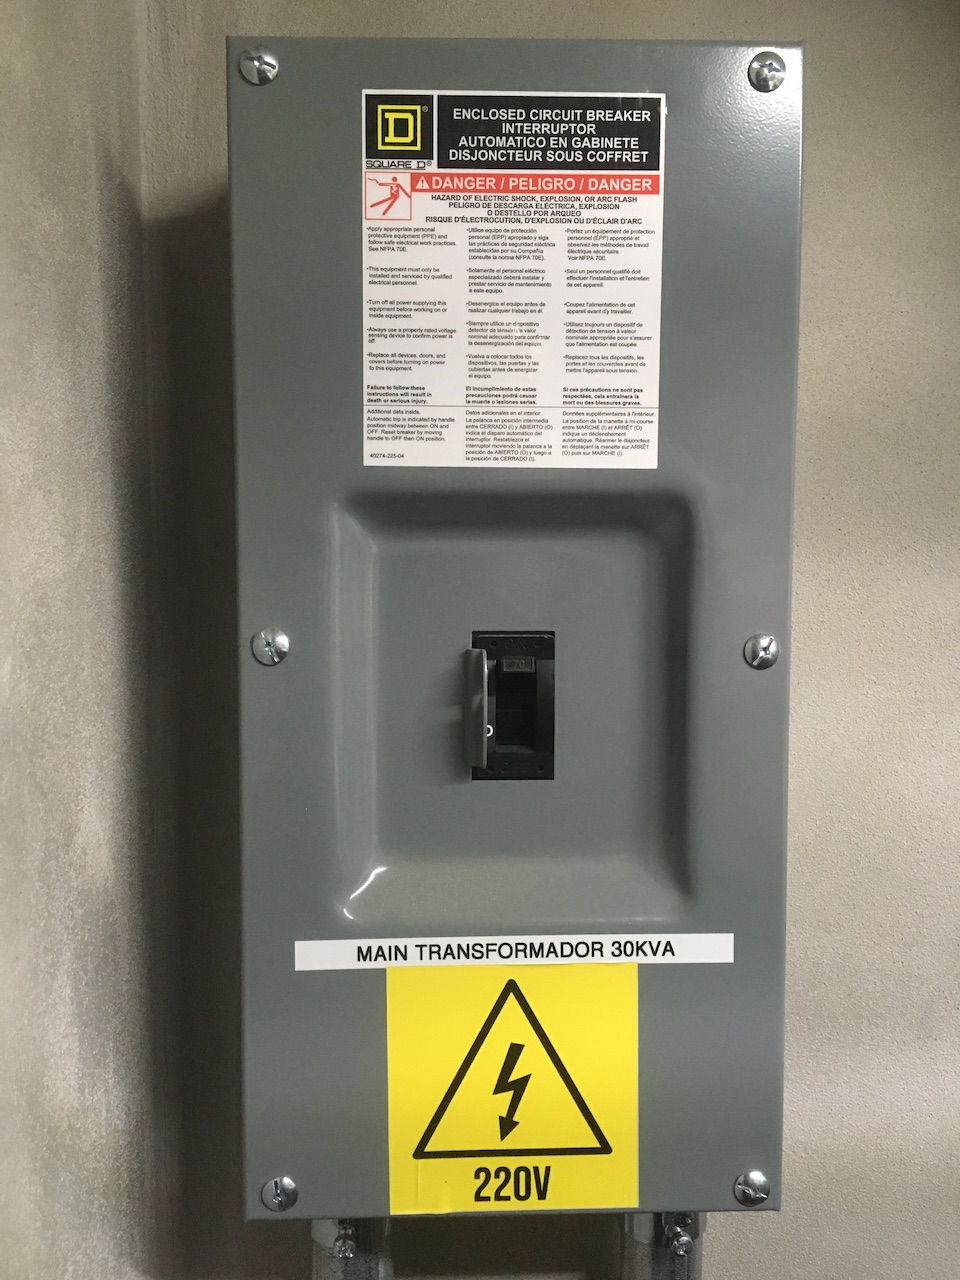
\includegraphics[width=0.45\linewidth,angle=0]{figures/electrical-power-ddoti-main-breaker-box.jpg}}
\arrowandlabel{(0.2,-1.0)}{(0,-5)}{north}{{\projectname} Main Breaker}
\end{labeled}
\end{center}
\caption{The main breaker box in shed.}
\label{figure:main-breaker-box}
\end{figure}
\fi

\section{Circuits}

\begin{figure}[t]
\ifcoatli
\begin{center}
\begin{labeled}{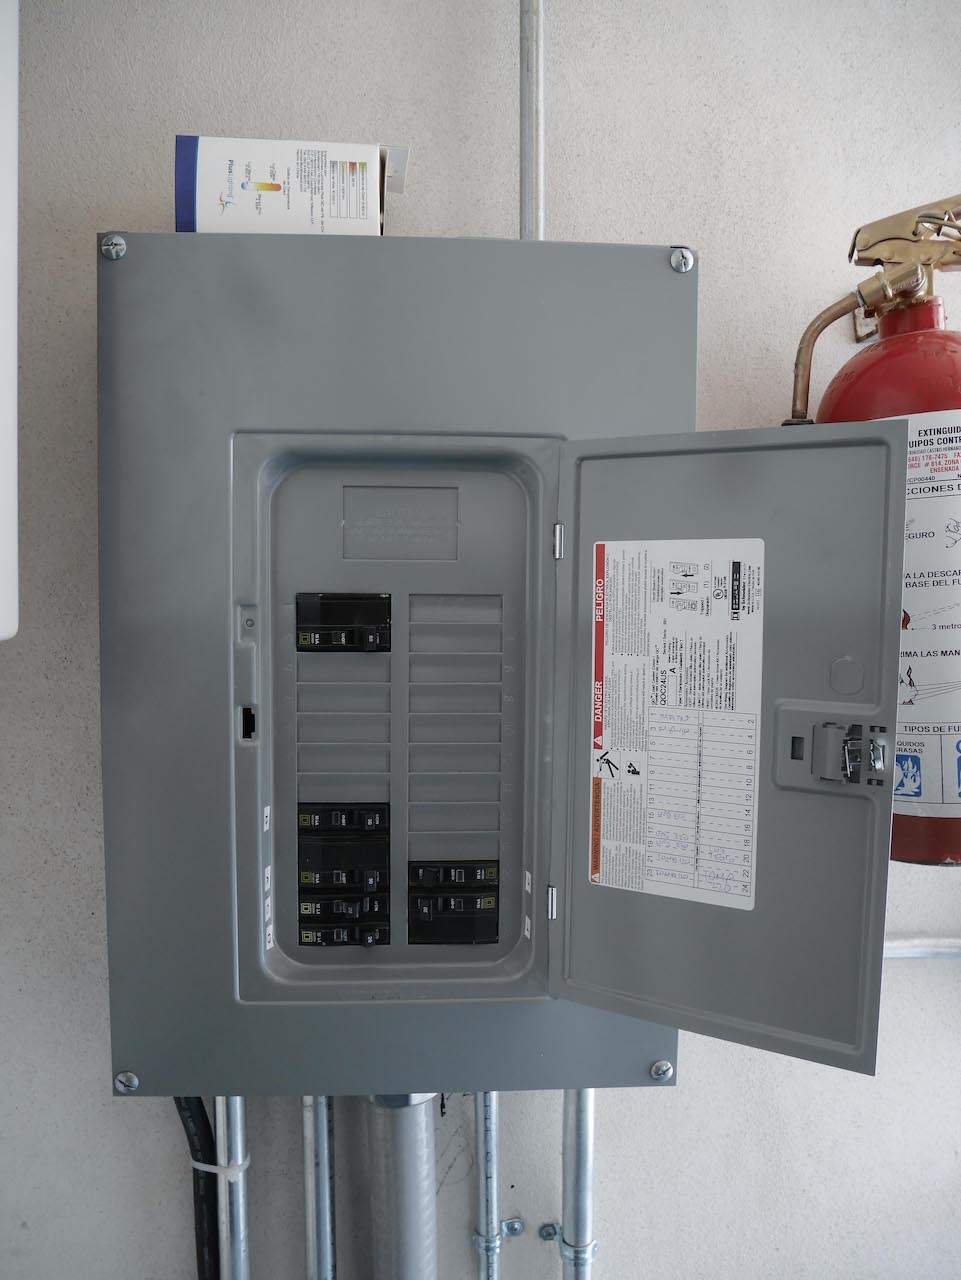
\includegraphics[height=0.7\linewidth]{figures/electrical-power-coatli-circuit-box.jpg}}
\arrowandlabel{(-0.7,0.5)}{(0,5)}{south}{Master Breaker}
\arrowandlabel{(-0.5,-2.2)}{(0,-5)}{north}{Breakers for Circuits A--F}
\end{labeled}
\end{center}
\caption{The circuit box the {\projectname} shed. The master breaker is at the top. The breakers for circuits A--F are at the bottom.}
\fi
\ifddoti
\begin{center}
\begin{labeled}{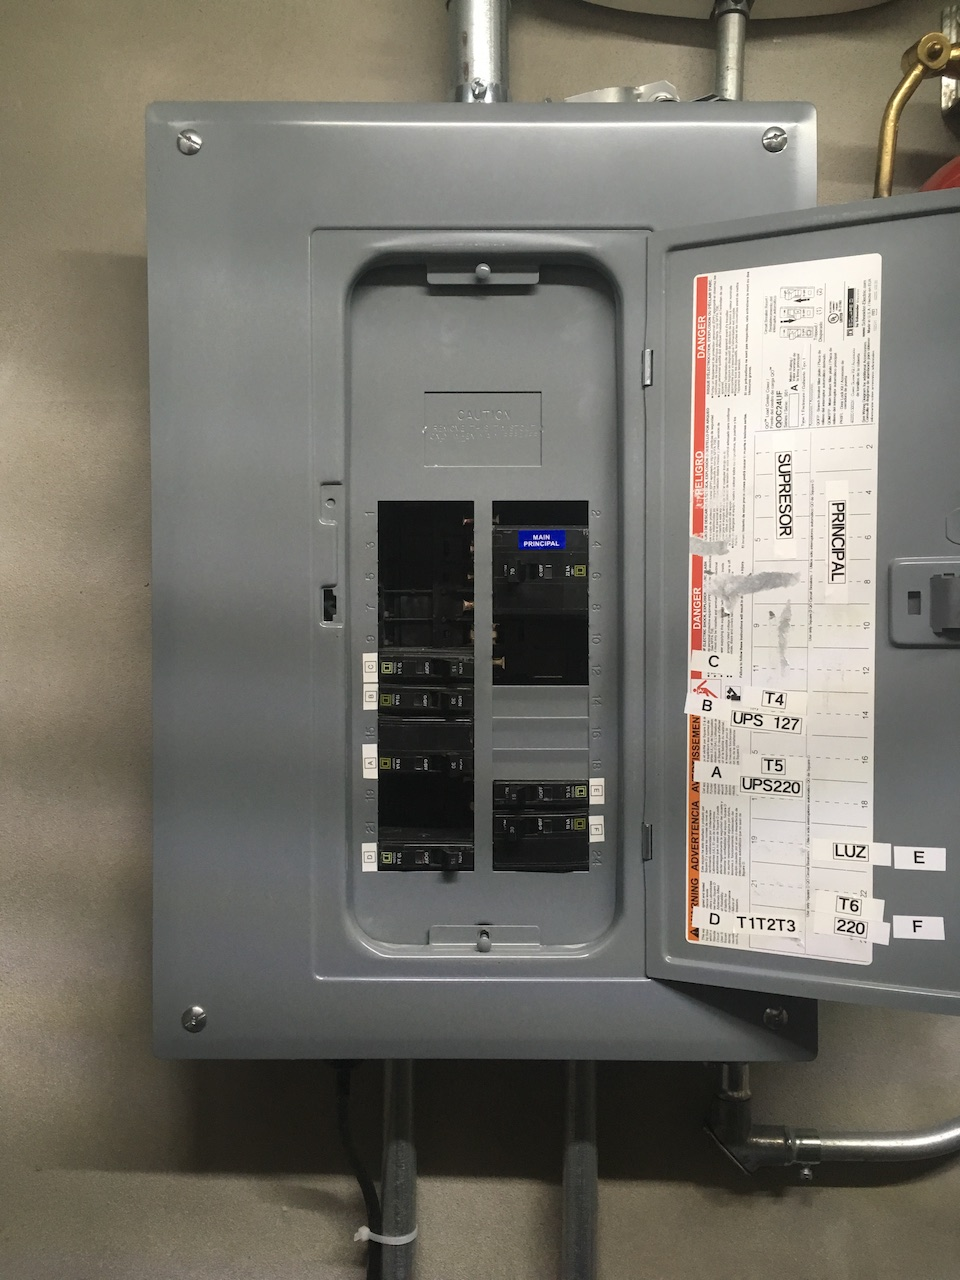
\includegraphics[width=0.45\linewidth,angle=0]{figures/electrical-power-ddoti-circuit-box.jpg}}
\arrowandlabel{(0.4,1)}{(0.5,5)}{south}{Master Breaker}
\arrowandlabel{(0,-1.7)}{(0,-5)}{north}{Breakers for Circuits A--F}
\end{labeled}
\end{center}
\caption{The circuit box the {\projectname} shed. The master breaker is at the top. The breakers for circuits A--F are at the bottom.}
\fi
\label{figure:circuit-box}
\end{figure}

Figure~\ref{figure:circuit-box} shows the circuit box in the shed. The master breaker is 80 A. The electricity supply is divided between the circuits listed in Table~\ref{table:circuits}, each with their own breaker. 

The 220~V circuits are generated between the two phases (L1 and L2). As a consequence, the 220~V circuits are live-live-ground, with 220~V between the two lives but each live 127~V above ground. (This is in contrast to a European-style live-neutral-ground 220~V circuit, with 220~V between live and neutral and with neutral nominally at the ground level.)

The 127~V circuits are generated between one of the two phases (L1 or L2) and the neutral (N). As a consequence, the 127~V circuits are live-neutral-ground, with 127~V between live and neutral and with neutral nominally at the ground level.

The wall sockets in the shed are labelled with their circuit.

Circuits A and B are regulated after the wall sockets by the two UPS units. The other circuits are unregulated. 

\begin{table*}
\caption{Circuits}
\label{table:circuits}
\begin{center}
\small
\resizebox{\columnwidth}{!}{
\begin{tabular}{lllll}
\hline
Circuit&Connection&Voltage&Breaker&Use\\
\hline
\ifcoatli
Master&L1-L2&220~V&80~A&Master for all circuits\\
A&L1-L2&220~V&30~A&Wall socket in shed for 220~V UPS (T5 $1\times$ NEMA L6-20R)\\
B&L2-N&127~V&30~A&Wall socket in shed for 127~V UPS (T4 $1\times$ NEMA L5-30R)\\
C&L1-N&127~V&20~A&Platform\\
D&L2-N&127~V&20~A&Wall sockets in shed (T0/T1/T2/T3 $2\times$ NEMA 5-15R)\\
E&L2-N&127~V&20~A&Lights in shed\\
F&L1-L2&220~V&30~A&Wall socket in shed (T6 $1\times$ NEMA L6-20R)\\
\fi
\ifddoti
Master&&220~V&70~A&Master for all circuits\\
A&L1-L2&220~V&30~A&Wall socket in shed for 220~V UPS (T5 $1\times$ NEMA L6-20R)\\
B&L2-N&127~V&30~A&Wall socket in shed for 127~V UPS (T4 $1\times$ NEMA L5-30R)\\
C&L1-N&127~V&15~A&Platform\\
D&L2-N&127~V&15~A&Wall sockets in shed (T1/T2/T3 $2\times$ NEMA 5-15R)\\
E&L2-N&127~V&15~A&Lights in shed\\
F&L1-L2&220~V&30~A&Wall socket in shed (T6 $1\times$ NEMA L6-20R)\\
\fi
\hline
\end{tabular}
}
\end{center}
\end{table*}

\section{UPS Units}

There are two UPS units in the rack in the shed. Both are Eaton 9310 models with nominal capacities of 3000~VA or 2700 W. Each is equipped with an external battery module, which extends the capacity to about 20 minutes of supply at full load.

\subsection{220~V UPS}

\begin{figure*}
\begin{center}
\footnotesize 
\resizebox{\columnwidth}{!}{
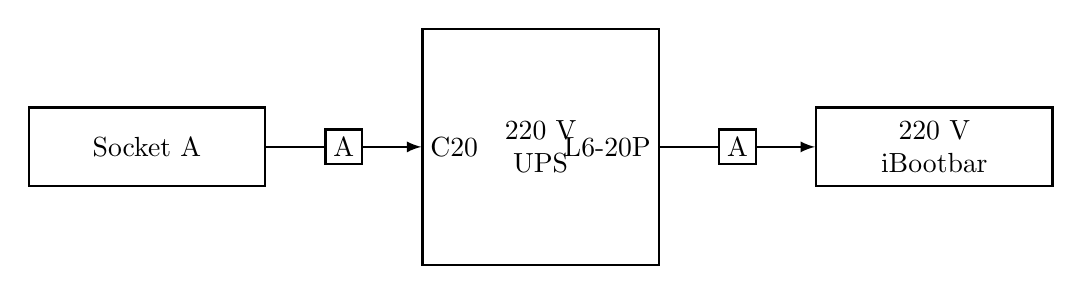
\begin{tikzpicture}
[
 thick,
 >={latex},
 align=center,
 inner sep=1mm,
 box/.style={draw=black,rectangle,minimum height=1cm,minimum width=3cm},
 main/.style={draw=black,rectangle,minimum width=3cm,minimum height=3cm},
 circuit/.style={draw=black,rectangle,fill=white}
]
\draw [white] (-6.5,0) -- (+6.5,0);
\node (ups-220) [main] at (0,0) {220 V\\ UPS};
\node (socket-a) at (-5,0) [box] {Socket A};
\node (ibb-220) at (+5,0) [box] {220 V\\iBootbar};
\draw[->] (socket-a) -- node [circuit] {A} (ups-220.west) node [right] {C20};
\draw[->] (ups-220.east) node [left] {L6-20P} -- node [circuit] {A} (ibb-220);
\end{tikzpicture}
}
\end{center}
\caption{Schematic of the Electrical Power Connections To and From the 220 V UPS}
\label{figure:schematic-electrical-power-box-ups-220}
\end{figure*}

The 220~V UPS is an Eaton PW9130G3000R-XL2U with PW9130N3000R-EBM2U external battery module. It is configured for 220~V 60~Hz input and output. Both the input and output are 220~V live-live-ground, with 220~V between the two lives and 127~V between each live and the ground.

Figure~\ref{figure:schematic-electrical-power-box-ups-220} shows a schematic of the electrical power connections.

The UPS is supplied via a NEMA L6-20P to C19 coupler connected to the NEMA L6-20R wall socket of circuit A and the C20 input socket of the UPS.

One of the NEMA L6-20R output sockets is connected to the 220~V iBootBar. No other output sockets are used.

If the UPS fails, it can be bypassed manually by connecting the NEMA L6-20P plug of the 220~V iBootBar to directly to the wall socket of circuit A.

\subsection{127~V UPS}

\begin{figure*}
\begin{center}
\footnotesize 
\resizebox{\columnwidth}{!}{
\begin{tikzpicture}[
 thick,
 >={latex},
 align=center,
 inner sep=1mm,
 box/.style={draw=black,rectangle,minimum height=1cm,minimum width=3cm},
 main/.style={draw=black,rectangle,minimum width=3cm,minimum height=3cm},
 circuit/.style={draw=black,rectangle,fill=white}
]
\draw [white] (-6.5,0) -- (+6.5,0);
\node (ups-127) [main] at (0,0) {127 V\\ UPS};
\node (socket-b) at (-5,0) [box] {Socket B};
\node (ibb-127) at (+5,+0.6) [box] {127 V\\iBootbar};
\node (rack-power-strip) at (+5,-0.6) [box] {Rack\\Power Strip};
\draw[->] (socket-b) -- node [circuit] {B} (ups-127);
\draw[->] 
 ($(ups-127.east) + (0,+0.9)$) node [left] {5-20R} 
 -- node [circuit] {B} 
 ($(ibb-127.west) + (0,+0.3)$);
\draw[->] 
 ($(ups-127.east) + (0,+0.3)$) node [left] {5-20R} 
 -- node [circuit] {B} 
 ($(ibb-127.west) + (0,-0.3)$);
\draw[->] 
 ($(ups-127.east) + (0,-0.6)$) node [left] {5-20R} 
 -- node [circuit] {B} 
 ($(rack-power-strip.west) + (0,0)$);
\end{tikzpicture}
}
\end{center}
\caption{Schematic of the Electrical Power Connections To and From the 127 V UPS}
\label{figure:schematic-electrical-power-box-ups-127}
\end{figure*}

The 127~V UPS is an Eaton PW9130L3000R-XL2U with PW9130N3000R-EBM2U external battery module. It is configured for 127~V 60~Hz input and output.

Figure~\ref{figure:schematic-electrical-power-box-ups-127} shows a schematic of the electrical power connections.

The UPS is supplied via a NEMA L5-30P plug connected to the NEMA L5-30R wall socket of circuit B.

Two of the NEMA 5-20R output sockets are connected to the NEMA 5-15P plugs of the 127~V iBootBar. Another NEMA 5-20R output socket is connected to the rack power strip. 

%The mount controller is \emph{not} connected via an iBootBar because it requires too much current. The power requirements of the mount controller are discussed on page 9 of the ASTELCO manual. The maximum draw in typical use is 400 W while tracking. However, it can use up to 1400 W when blocked. ASTELCO recommend fusing to 2500 W to cover the initial transient load. At 127 V, this corresponds to 20 A.
%The 127~V iBootBar is a 2N15-M model and can supply up to 12 A or 1500 W. This is insufficient for the initial transient.

If the UPS fails, it can be bypassed manually by connecting the two NEMA 5-15P plugs of the 127~V iBootBar directly to the wall sockets of circuit D.

\section{iBootBars}

There are two iBootBars in the rack in the shed, one 127~V and one 220~V. Both are the connected to the corresponding 127~V and 220~V UPS units. They are physically located in the rear of the rack towards the top.

\subsection{220~V iBootBar}

\begin{figure*}
\begin{center}
\footnotesize 
\resizebox{\columnwidth}{!}{
\begin{tikzpicture}
[
 thick,
 >={latex},
 align=center,
 inner sep=1mm,
 box/.style={draw=black,rectangle,minimum height=1cm,minimum width=3cm},
 main/.style={draw=black,rectangle,minimum width=3cm,minimum height=3cm},
 circuit/.style={draw=black,rectangle,fill=white}
]
\draw [white] (-6.5,0) -- (+6.5,0);
\node (ibb-220) [main] at (0,0) {220 V\\iBootBar};
\node (ups-220) at (-5,0) [box] {220 V\\UPS};
\ifcoatli
\node (secondary) at (5,+0.6) [box] {Secondary\\Controller};
\node (enclosure) at (5,-0.6) [box] {Enclosure\\Controller};
\draw[<-] (secondary.west) -- node [circuit] {A} +(-2,0) node [left] {F};
\draw[<-] (enclosure.west) -- node [circuit] {A} +(-2,0) node [left] {F};
\fi
\ifddoti
\node (enclosure) at (5,0) [box] {Enclosure\\Controller};
\draw[<-] (enclosure.west) -- node [circuit] {A} +(-2,0) node [left] {F};
\fi
\draw[->] (ups-220) -- node [circuit] {A} (ibb-220.west) node [right] {C20};
\end{tikzpicture}
}
\end{center}
\caption{Schematic of the Electrical Power Connections To and From the 220 V iBootBar}
\label{figure:schematic-electrical-power-box-ibb-220}
\end{figure*}

This is a DataProbe iBootBar iBB-C20. Figure~\ref{figure:schematic-electrical-power-box-ibb-220} shows a schematic of the electrical power connections.

The C20 input socket is connected to the 220~V UPS unit with a cable with C19 and NEMA L6-20P plugs.

The connections to the type F output sockets (“C13 female”) are given in Table~\ref{table:ibbs}. The iBootBar can supply up to 20~A.

The iBootBar is connected to the LAN at the address given in Table~\ref{table:network-addresses}. The HTTP and telnet account names and passwords are “{\projectaccount}” and “{\projectaccount}”. The HTTP interface is available from the {\projectname} web interface home page.

\subsection{127~V iBootBar}

\begin{figure*}
\begin{center}
\footnotesize 
\resizebox{\columnwidth}{!}{
\begin{tikzpicture}
[
 thick,
 >={latex},
 align=center,
 inner sep=1mm,
 box/.style={draw=black,rectangle,minimum height=1cm,minimum width=3cm},
 main/.style={draw=black,rectangle,minimum width=3cm,minimum height=3cm},
 circuit/.style={draw=black,rectangle,fill=white}
]
\draw [white] (-6.5,0) -- (+6.5,0);
\node (ibb-127) [main,minimum height=9.4cm] at (0,0) {127 V\\iBootBar};
\node (ups-127) at (-5,0) [box] {127 V\\UPS};
\draw[->] (-3.5,+0.3) -- node [circuit] {B} (-1.5,+0.3);
\draw[->] (-3.5,-0.3) -- node [circuit] {B} (-1.5,-0.3);
\node (cable-b1) [box] at (5,+4.2) {Platform (Cable B1)};
\node (cable-b2) [box] at (5,+3.0) {Instrument (Cable B2)};
\node (serial) [box] at (5,+1.8) {Serial Adapter};
\node (mount) [box] at (5,+0.6) {Mount};
\node (access) [box] at (5,-0.6) {\ttfamily access};
\node (firewall) [box] at (5,-1.8) {\ttfamily firewall};
\node (services) [box] at (5,-3.0) {\ttfamily services};
\node (control) [box] at (5,-4.2) {\ttfamily control};

\draw[->] 
 ($(ibb-127.east) + (0,4.2)$) node [left] {5-15R} 
 -- ++(1,0) node [circuit] {B1} 
 |- (cable-b1.west);
\draw[->]
($(ibb-127.east) + (0,+3.0)$) node [left] {5-15R} 
 -- ++(1,0) node [circuit] {B2} 
 |- (cable-b2.west);
\draw[->] 
 ($(ibb-127.east) + (0,+1.8)$) node [left] {5-15R} 
 -- ++(1,0) node [circuit] {B} 
 |- (serial.west);
\draw[->] 
 ($(ibb-127.east) + (0,+0.6)$) node [left] {5-15R} 
 -- ++(1,0) node [circuit] {B} 
 |- (mount.west);
\draw[->] 
 ($(ibb-127.east) + (0,-0.6)$) node [left] {5-15R} 
 -- ++(1,0) node [circuit] {B} 
 |- (access.west);
\draw[->] 
 ($(ibb-127.east) + (0,-1.8)$) node [left] {5-15R} 
 -- ++(1,0) node [circuit] {B} 
 |- (firewall.west);
\draw[->] 
 ($(ibb-127.east) + (0,-3.0)$) node [left] {5-15R} 
 -- ++(1,0) node [circuit] {B} 
 |- (services.west);
\draw[->] 
 ($(ibb-127.east) + (0,-4.2)$) node [left] {5-15R} 
 -- ++(1,0) node [circuit] {B} 
 |- (control.west);
\end{tikzpicture}
}
\end{center}
\caption{Schematic of the Electrical Power Connections To and From the 127 V iBootBar}
\label{figure:schematic-electrical-power-box-ibb-127}
\end{figure*}

This is a DataProbe iBootBar iBB-2N15-M.  Figure~\ref{figure:schematic-electrical-power-box-ibb-127} shows a schematic of the electrical power connections.

The two NEMA 5-15P input plugs are connected to the 127~V UPS unit. 

The connections to the NEMA 5-15R output sockets are given in Table~\ref{table:ibbs}. The iBootBar can supply up to 15~A to each bank of four output sockets.

The iBootBar is connected to the LAN at the address given in Table~\ref{table:network-addresses}. The HTTP and telnet account names and passwords are “{\projectaccount}” and “{\projectaccount}”. The HTTP interface is available from the {\projectname} web interface home page.

The modem facility is not used.

TODO: Configure watchdog.

\begin{table*}
\caption{iBootBar Output Sockets}
\label{table:ibbs}
\begin{center}
\begin{tabular}{lll}
\hline
Socket&220~V iBootBar&127~V iBootBar\\
\hline
1&Enclosure&Platform (Cable B1)\\
2&
\ifcoatli
Secondary
\fi
\ifddoti
-
\fi
&\verb|access|\\
3&-&Instrument (Cable B2)\\
5&-&Mount\\
5&-&\verb|firewall|\\
6&-&\verb|services|\\
7&-&\verb|control|\\
8&-&\verb|serial|\\
\hline
\end{tabular}
\end{center}
\end{table*}

\section{Rack Power Strip}

%\begin{figure*}
%\begin{center}
%\footnotesize 
%\resizebox{\columnwidth}{!}{
%\begin{tikzpicture}
%[
% thick,
% >={latex},
% align=center,
% inner sep=1mm,
% box/.style={draw=black,rectangle,minimum height=1cm,minimum width=3cm},
% main/.style={draw=black,rectangle,minimum width=3cm,minimum height=3cm},
% circuit/.style={draw=black,rectangle,fill=white}
%]
%\draw [white] (-6.5,0) -- (+6.5,0);
%\node (power-strip) [main] at (0,0) {Power\\Strip};
%\node (ibb-127) at (-5,0) [box] {127 V\\iBootBar};
%\draw[->] (ibb-127) -- node [circuit] {B} (power-strip);
%
%\node (fiber-adapter) [box] at (5,+3.6) {Fiber Adapter};
%\node (time-capsule) [box] at (5,+2.4) {Time Capsule};
%\node (switch) [box] at (5,+1.2) {Switch};
%\node (control-mac) [box] at (5,+0.0) {Control Mac};
%\node (data-mac) [box] at (5,-1.2) {Data Mac};
%\node (pc) [box] at (5,-2.4) {PC};
%\node (monitor) [box] at (5,-3.6) {Monitor};
%\draw[->] 
% ($(power-strip.east) + (0,+1.2)$) node [left] {5-15R} 
% -- +(0.5,0) node [circuit] {B} 
% -- +(1.0,0) 
% |- (fiber-adapter.west);
%\draw[->] 
% ($(power-strip.east) + (0,+0.8)$) node [left] {5-15R} 
% -- +(1.0,0) node [circuit] {B} 
% -- +(1.3,0) 
% |- (time-capsule.west);
%\draw[->] 
% ($(power-strip.east) + (0,+0.4)$) node [left] {5-15R} 
% -- +(0.5,0) node [circuit] {B} 
% -- +(1.6,0) 
% |- (switch.west);
%\draw[->] 
% ($(power-strip.east) + (0,+0.0)$) node [left] {5-15R} 
% -- +(1.0,0) node [circuit] {B} 
% -- (control-mac.west);
%\draw[->] 
% ($(power-strip.east) + (0,-0.4)$) node [left] {5-15R} 
% -- +(0.5,0) node [circuit] {B} 
% -- +(1.6,0) 
% |- (data-mac.west);
%\draw[->] 
% ($(power-strip.east) + (0,-0.8)$) node [left] {5-15R} 
% -- +(1.0,0) node [circuit] {B} 
% -- +(1.3,0) 
% |- (pc.west);
%\draw[->] 
% ($(power-strip.east) + (0,-1.2)$) node [left] {5-15R} 
% -- +(0.5,0) node [circuit] {B} 
% -- +(1.0,0) 
% |- (monitor.west);
%\end{tikzpicture}
%}
%\end{center}
%\caption{Schematic of the Electrical Power Connections To and From the Rack Power Strip}
%\label{figure:schematic-electrical-power-rack-power-strip}
%\end{figure*}

At the rear of the rack, adjacent to the 127~V iBootBar, is a 8-way NEMA 5-15R power strip. The power strip powers the computers and network equipment in the rack. The entire power strip, and hence all of the connected equipment, is directly supplied by the 127~V UPS.

%Figure~\ref{figure:schematic-electrical-power-rack-power-strip} shows a schematic of the electrical power connections.


%\section{Box A}
%
%\begin{figure*}
%\begin{center}
%\footnotesize 
%\resizebox{\columnwidth}{!}{
%\begin{tikzpicture}[
% thick,
% >={latex},
% align=center,
% inner sep=1mm,
% box/.style={draw=black,rectangle,minimum height=1cm,minimum width=3cm},
% main/.style={draw=black,rectangle,minimum width=3cm,minimum height=3cm},
% circuit/.style={draw=black,rectangle,fill=white}
%]
%\draw [white] (-6.5,0) -- (+6.5,0);
%\node (box-a) [main] at (0,0) {Box A};
%\node (ibb-127) at (-5,+0.0) [box] {127 V\\iBootBar};
%\draw[->] (ibb-127.east) -- node [circuit] {B} +(2,0) node [right] {C14};
%\end{tikzpicture}
%}
%\end{center}
%\caption{Schematic of the Electrical Power Connections To Box A}
%\label{figure:schematic-electrical-power-box-a}
%\end{figure*}
%
%Box A is a smart control box located in the shed.  Figure~\ref{figure:schematic-electrical-power-box-a} shows a schematic of the electrical power connections to Box A.
%
%Box A is connected to circuit B, which powers the electronics, internal heater, and internal fans in Box A. 
%
%The connection to circuit B is via a NEMA 5-15P to C13 cable. The NEMA 5-15P plug is connected to an output socket of the 127 V iBootBar and the C13 plug is connected to the C14 input socket on Box A.
%
%Circuit B is switched and fuzed with a 1~A fuze at the entrance to Box A.

\begin{table*}
\caption{Fuzes}
\label{table:fuzes}
\begin{center}
\begin{tabular}{lcc}
\hline
Location&Circuit&Fuze\\
\hline
\ifcoatli
Power Box&B1\phantom{}&\phantom{0}3 A\\
Power Box&B2\phantom{}&\phantom{0}3 A\\
Power Box&C\phantom{0}&\phantom{}15 A\\
Platform Box&B1\phantom{}&\phantom{0}3 A\\
Instrument Box&B2\phantom{}&\phantom{0}3 A\\
\fi
\ifddoti
Power Box&B1\phantom{}&\phantom{0}3 A\\
Power Box&B2\phantom{}&\phantom{}15 A\\
Power Box&C\phantom{0}&\phantom{}15 A\\
Platform Box&B1\phantom{}&\phantom{0}3 A\\
Instrument0 Box&B2\phantom{}&\phantom{0}3 A\\
Instrument1 Box&B2\phantom{}&\phantom{0}3 A\\
\fi
\hline
\end{tabular}
\end{center}
\end{table*}


\section{Power Box}

\begin{figure*}
\begin{center}
\footnotesize 
\resizebox{\columnwidth}{!}{
\begin{tikzpicture}[
 thick,
 >={latex},
 align=center,
 inner sep=1mm,
 box/.style={draw=black,rectangle,minimum height=1cm,minimum width=3cm},
 main/.style={draw=black,rectangle,minimum width=3cm,minimum height=3cm},
 circuit/.style={draw=black,rectangle,fill=white}
]
\draw [white] (-6.5,0) -- (+6.5,0);
\ifcoatli
\node (power-box) [main,minimum height=5.8cm] at (0,0) {Power Box};
\fi
\ifddoti
\node (power-box) [main,minimum height=4.6cm] at (0,0) {Power Box};
\fi
\node (ibb-127) at (-5,+0.6) [box] {127 V\\iBootBar};
\node (circuit-box) at (-5,-0.6) [box] {Circuit Box};
\draw[->] (-3.5,+0.9) -- node [circuit] {B1} +(+2,0);
\draw[->] (-3.5,+0.3) -- node [circuit] {B2} +(+2,0);
\draw[->] (circuit-box.east) -- node [circuit] {C} +(+2,0);
\node at ($(power-box.north) + (-0.5,0)$) [below] {5-15R};
\node at ($(power-box.north) + (+0.5,0)$) [below] {5-15R};
\node at ($(power-box.north) + (0,-0.4)$) [below] {Sockets C};
\ifcoatli
\node (instrument1-box) at (+5,+2.4) [box] {Box E};
\node (instrument-box) at (+5,+1.2) [box] {Box D};
\node (platform-box) at (+5,+0.0) [box] {Platform Box};
\node (manual-light) at (+5,-1.2) [box] {Manual Light};
\node (emergency-light) at (+5,-2.4) [box] {Emergency Light};
\fi
\ifddoti
\node (platform-box) at (+5,+0.6) [box] {Platform Box};
\node (instrument0-box) at (+5,+1.8) [box] {Instrument0 Box};
\node (instrument1-box) at (+5,+3.0) [box] {Instrument1 Box};
\node (manual-light) at (+5,-0.6) [box] {Manual Light};
\node (emergency-light) at (+5,-1.8) [box] {Emergency Light};
\draw[<-] (instrument0-box.west) -- +(-1,0) node [circuit] {B2} -- +(-2,0);
\draw[->] (instrument0-box.east) -- +(0.4,0) -- node [circuit] {B2} +(0.4,+1.2) |- (instrument1-box.east);
\fi
\ifcoatli
\draw[<-] (instrument-box.west) -- +(-1,0) node [circuit] {B1} -- +(-2,0);
\fi
\draw[<-] ($(platform-box.west) + (0,+0.3)$) -- +(-1,0) node [circuit] {B1} -- +(-2,0);
\draw[<-] ($(platform-box.west) + (0,-0.3)$) -- +(-1,0) node [circuit] {C} -- +(-2,0);
\draw[<-] (manual-light.west) -- +(-1,0) node [circuit] {C} -- +(-2,0);
\draw[<-] (emergency-light.west) -- +(-1,0) node [circuit] {C} -- +(-2,0);
\end{tikzpicture}
}
\end{center}
\caption{Schematic of the Electrical Power Connections To and From the Power Box}
\label{figure:schematic-electrical-power-power-box}
\end{figure*}

The power box is a dumb electrical distribution box located on the platform.  Figure~\ref{figure:schematic-electrical-power-power-box} shows a schematic of the electrical power connections to Power Box.

The power box is connected to circuits B1, B2, and C. Circuits B1 and B2 are subcircuits of circuit B. Circuit B1 is used to power electronics, internal heaters, and internal fans in Boxes C and D, the two other boxes on the platform. Circuit B2 is used for power the electronics, internal heaters, and internal fans in Box E on the telescope. Circuit C is used to power the two NEMA 5-15R plugs on the power box (for general use), the three lights on the platform (one with manual control, one with manual/electronic control, and one emergency), and the external heater on the platform.

The connection to circuits B1 and B2 are via cables with NEMA 5-15P plugs connected to the 127~V iBootBar. 

The connection to circuit C is hardwired to the circuit box in the shed. The connections are hardwired at the power box.

The three circuits are switched and fuzed (see Table~\ref{table:fuzes}) at the entrance to the power box.

The manually-controlled light is hardwired to the platform box and has a manual switch on the power box.

\section{Platform Box}

\begin{figure*}
\begin{center}
\footnotesize 
\resizebox{\columnwidth}{!}{
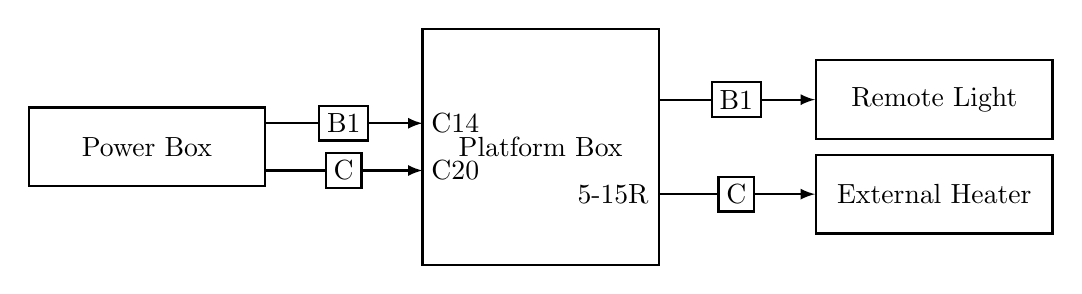
\begin{tikzpicture}[
 thick,
 >={latex},
 align=center,
 inner sep=1mm,
 box/.style={draw=black,rectangle,minimum height=1cm,minimum width=3cm},
 main/.style={draw=black,rectangle,minimum width=3cm,minimum height=3cm},
 circuit/.style={draw=black,rectangle,fill=white}
]
\draw [white] (-6.5,0) -- (+6.5,0);
\node (platform-box) [main] at (0,0) {Platform Box};
\node (power-box) [box] at (-5,0) {Power Box};
\node (light) at (+5,+0.6) [box] {Remote Light};
\node (heater) at (+5,-0.6) [box] {External Heater};
\draw[->] (-3.5,+0.3) -- node [circuit] {B1} +(2,0) node [right] {C14};
\draw[->] (-3.5,-0.3) -- node [circuit] {C} +(2,0) node [right] {C20};
\draw[<-] (light.west) -- node [circuit] {B1} +(-2,0);
\draw[<-] (heater.west) -- node [circuit] {C} +(-2,0) node [left] {5-15R};
\end{tikzpicture}
}
\end{center}
\caption{Schematic of the Electrical Power Connections To and From the Platform Box}
\label{figure:schematic-electrical-power-platform-box}
\end{figure*}

The platform box is a smart control box located on the platform. Figure~\ref{figure:schematic-electrical-power-platform-box} shows a schematic of the electrical power connections to the platform box.


The platform box is connected to circuits B1 and C. Circuit B1 is a subcircuit of circuit B. Circuit B1 is used to power the electronics, the internal heater, and the internal fans. Circuit C is used to power an external light and the external heater on the platform.

The connection to circuit B1 is via a cable with a C13 plug that connects to the C14 input socket on the platform box. The cable is hardwired to the power box.

The connection to circuit C is via a cable with a C19 plug that connects to the C20 input socket on the platform box. The cable is hardwired to the power box.

The connections to the manually/electronically-controlled light and heater are via the two NEMA 5-15R sockets on the platform box. The light is controlled both by a relay and by a manual switch on the platform box (with the light being on if either the relay or manual switch are on). The heater is controlled by a relay.

Circuit B1 is switched and fuzed (see Table~\ref{table:fuzes}) at the entrance to the platform box.

\ifcoatli

\section{Instrument Box}

\begin{figure*}
\begin{center}
\footnotesize 
\resizebox{\columnwidth}{!}{
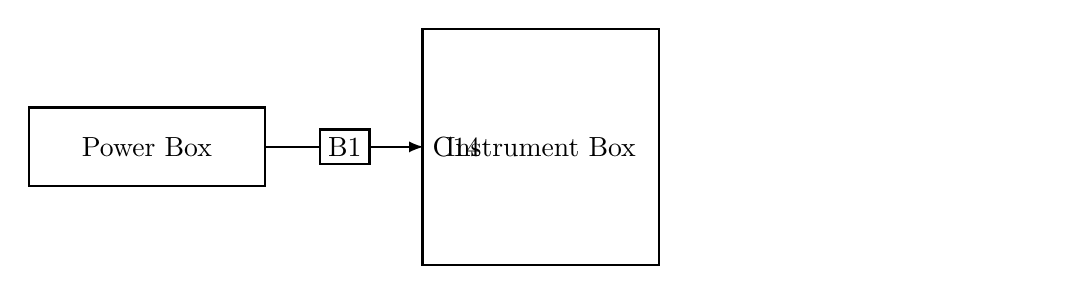
\begin{tikzpicture}[
 thick,
 >={latex},
 align=center,
 inner sep=1mm,
 box/.style={draw=black,rectangle,minimum height=1cm,minimum width=3cm},
 main/.style={draw=black,rectangle,minimum width=3cm,minimum height=3cm},
 circuit/.style={draw=black,rectangle,fill=white}
]
\draw [white] (-6.5,0) -- (+6.5,0);
\node (instrument-box) [main] at (0,0) {Instrument Box};
\node (power-box) [box] at (-5,0) {Power Box};
\draw[->] (power-box.east) -- node [circuit] {B1} +(2,0) node [right] {C14};
\end{tikzpicture}
}
\end{center}
\caption{Schematic of the Electrical Power Connections To Instrument Box}
\label{figure:schematic-electrical-power-instrument-box}
\end{figure*}

The instrument box is a smart control box located on the platform. Figure~\ref{figure:schematic-electrical-power-instrument-box} shows a schematic of the electrical power connections to Box D.

The instrument nox is connected to circuit B1. Circuit B1 is a subcircuit of circuit B. Circuit B1 is used to power the electronics, the internal heater, and the internal fans.

The connection to circuit B1 is via a cable with a C13 plug that connects to the C14 input socket on the platform box. The cable is hardwired to the power box.

Circuit B1 is switched and fuzed (see Table~\ref{table:fuzes}) at the entrance to the instrument box.

\section{Box E}

\begin{figure*}
\begin{center}
\footnotesize 
\resizebox{\columnwidth}{!}{
\begin{tikzpicture}[
 thick,
 >={latex},
 align=center,
 inner sep=1mm,
 box/.style={draw=black,rectangle,minimum height=1cm,minimum width=3cm},
 main/.style={draw=black,rectangle,minimum width=3cm,minimum height=3cm},
 circuit/.style={draw=black,rectangle,fill=white}
]
\draw [white] (-6.5,0) -- (+6.5,0);
\node (instrument1-box) [main] at (0,0) {Box E};
\node (power-box) [box] at (-5,0) {Power Box};
\draw[->] (power-box.east) -- node [circuit] {B2} +(2,0) node [right] {C14};
\end{tikzpicture}
}
\end{center}
\caption{Schematic of the Electrical Power Connections To Box E}
\label{figure:schematic-electrical-power-instrument1-box}
\end{figure*}

Box E is a smart control box located on the pillar of the COATLI telescope. Figure~\ref{figure:schematic-electrical-power-instrument1-box} shows a schematic of the electrical power connections to Box E.

Box E is connected to circuit B2. Circuit B2 is a subcircuit of circuit B. Circuit B2 is used to power the electronics, the internal heater, and the internal fans.

The connection to circuit B2 is via a cable with a C13 plug that connects to the C14 input socket on Box E. The cable is hardwired to the power box.

Circuit B2 is switched and fuzed (see Table~\ref{table:fuzes}) at the entrance to Box E.

\fi

\ifddoti

\section{Instrument0 Box}

\begin{figure*}
\begin{center}
\footnotesize 
\resizebox{\columnwidth}{!}{
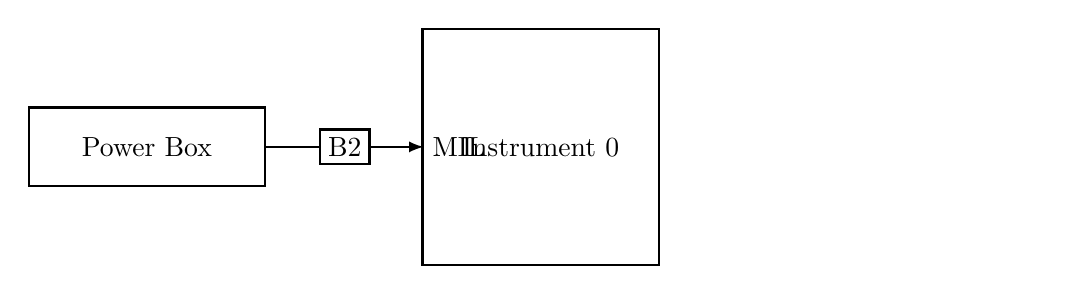
\begin{tikzpicture}[
 thick,
 >={latex},
 align=center,
 inner sep=1mm,
 box/.style={draw=black,rectangle,minimum height=1cm,minimum width=3cm},
 main/.style={draw=black,rectangle,minimum width=3cm,minimum height=3cm},
 circuit/.style={draw=black,rectangle,fill=white}
]
\draw [white] (-6.5,0) -- (+6.5,0);
\node (instrument0-box) [main] at (0,0) {Instrument 0};
\node (instrument1-box) [box] at (-5,0) {Power Box};
\draw[->] (instrument1-box.east) -- node [circuit] {B2} +(2,0) node [right] {MIL};
\end{tikzpicture}
}
\end{center}
\caption{Schematic of the Electrical Power Connections To The Instrument0 Box}
\label{figure:schematic-electrical-power-instrument0-box}
\end{figure*}

The instrument0 box is a smart control box located on the DDOTI telescopes. Figure~\ref{figure:schematic-electrical-power-instrument0-box} shows a schematic of the electrical power connections to the instrument0 box.

The instrument 0 box is connected to circuit B2. Circuit B2 is a subcircuit of circuit B. Circuit B2 is used to power the electronics, the internal heater, and the internal fans.

The connection to circuit B2 is via a cable with a MIL plug that connects to the MIL input socket on Box D. The cable is hardwired to the power box. The cable passes from the power box up onto the telescope through the mount and the custom connector.

Circuit B2 is switched and fuzed (see Table~\ref{table:fuzes}) at the entrance to the instrument0 box.

\section{The Instrument1 Box}

\begin{figure*}
\begin{center}
\footnotesize 
\resizebox{\columnwidth}{!}{
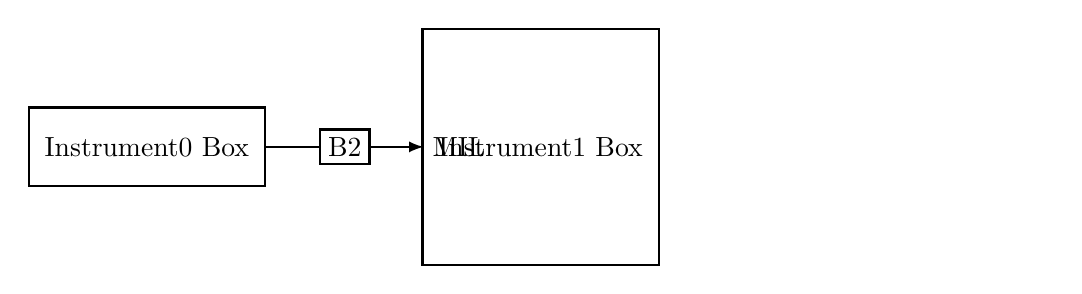
\begin{tikzpicture}[
 thick,
 >={latex},
 align=center,
 inner sep=1mm,
 box/.style={draw=black,rectangle,minimum height=1cm,minimum width=3cm},
 main/.style={draw=black,rectangle,minimum width=3cm,minimum height=3cm},
 circuit/.style={draw=black,rectangle,fill=white}
]
\draw [white] (-6.5,0) -- (+6.5,0);
\node (instrument1-box) [main] at (0,0) {Instrument1 Box};
\node (instrument0-box) [box] at (-5,0) {Instrument0 Box};
\draw[->] (instrument0-box.east) -- node [circuit] {B2} +(2,0) node [right] {MIL};
\end{tikzpicture}
}
\end{center}
\caption{Schematic of the Electrical Power Connections To Instrument1 Box}
\label{figure:schematic-electrical-power-instrument1-box}
\end{figure*}

The instrument1 box is a smart control box located on the pillar of the COATLI telescope. Figure~\ref{figure:schematic-electrical-power-instrument1-box} shows a schematic of the electrical power connections to Box E.

The instrument1 box is connected to circuit B2. Circuit B2 is a subcircuit of circuit B. Circuit B2 is used to power the electronics, the internal heater, and the internal fans.

The connection to circuit B2 is via a cable with a MIL plug that connects to the MIL input socket on the instrument1 box. The cable passes through the mount declination bearing to the instrument0 box and has an inline C13/C14 connector close to instrument0 box to allow instrument0 to be demounted.

Circuit B2 is switched and fuzed (see Table~\ref{table:fuzes}) at the entrance to Box E.

\fi

\section{Trouble-Shooting}

\begin{itemize}
\item Check cables. Has one been disconnected or worked itself lose?
\item Check switches. Is the equipment switched on? The smart boxes have switch for their regulated input (circuits B, B1, or B2). The power box has switches for circuits B1, B2, and C. The Macs and the PC have power switches. The ASTELCO equipment has power switches.
\item Check fuzes. Has one blown? See Table~\ref{table:fuzes}.
\item For circuits connected via an iBootBar (A, B, B1, and B2), check that the corresponding output socket is on. The state of the output sockets is given by the row of 8 green LEDs on the front of each iBootBar.
\item The emergency lights come on if the corresponding circuit (C for the platform and E for the shed) has no power. This can happen because a breaker trips or because the OAN mains supply has failed.
\item For circuits not connected via a UPS unit (C, D, E, and F), check that the OAN mains supply is working.
\item For circuits connected via a UPS unit (A, B, B1, and B2), check that the corresponding UPS is working.
\item Check the breakers in the circuit box in the shed. Has one tripped?
\ifcoatli
\item Check the breaker in the main breaker box in the 84-cm. Has it tripped?
\fi
\ifddoti
\item Check the breaker in the main breaker box. Has it tripped?
\fi
\item Check the equipment has not failed.
\end{itemize}

\section{Bibliography}

\begin{flushleft}
\begin{itemize}
\item “\href{bibliography/eaton-9130-ups.pdf}{Eaton 9300 UPS 700/3000~VA User's Guide}” (Revision 8)
\item “\href{bibliography/dataprobe-ibootbar.pdf}{iBootBar Installations and Operations}” (Version 1.5)
\end{itemize}
\end{flushleft}

